\documentclass[11pt, oneside]{article}   	% use "amsart" instead of "article" for AMSLaTeX format
\usepackage{geometry}                		% See geometry.pdf to learn the layout options. There are lots.
\geometry{letterpaper}                   		% ... or a4paper or a5paper or ... 
%\geometry{landscape}                		% Activate for for rotated page geometry
%\usepackage[parfill]{parskip}    		% Activate to begin paragraphs with an empty line rather than an indent
\usepackage{graphicx}				% Use pdf, png, jpg, or eps� with pdflatex; use eps in DVI mode
								% TeX will automatically convert eps --> pdf in pdflatex		
\usepackage{amssymb}
\usepackage{amsmath}
\usepackage{parskip}
\usepackage{color}

\title{Title}
%\author{The Author}
%\section{}
%\subsection*{}
\date{}							% Activate to display a given date or no date

\graphicspath{{/Users/telliott_admin/Dropbox/Tex/png/}}
% \begin{center} 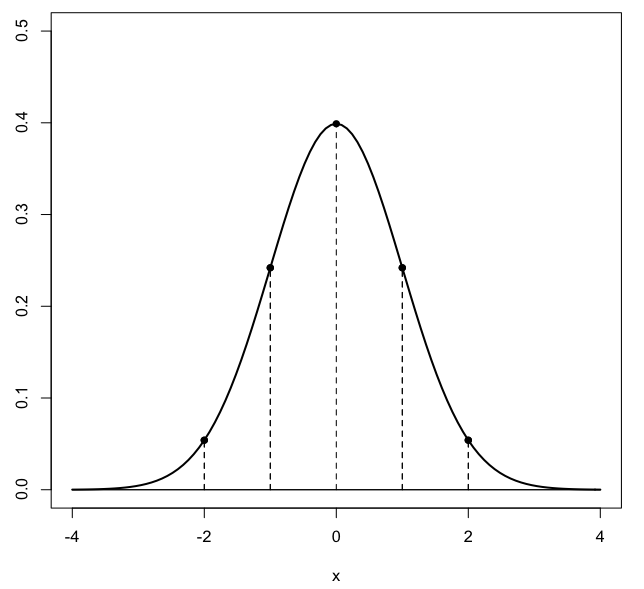
\includegraphics [scale=0.4] {gauss3.png} \end{center}
\begin{document}
\maketitle
\Large
Rotation of coordinates

The simplest way to get the formulas is to think about how to rotate the unit vectors by an angle $\phi$ counter-clockwise.  If we analyze this problem the question is, what values for $a$ and $c$ give a matrix will multiply $\mathbf{i}$ to give this result?
\[
\begin{bmatrix}  
a & b  \\  
c & d  
\end{bmatrix}
\begin{bmatrix}  
1  \\  
0  
\end{bmatrix}
=
\begin{bmatrix}  
\cos\  \phi  \\  
\sin\  \phi  
\end{bmatrix}
\]
Similarly, what values for $b$ and $d$ give a matrix which will multiply $\mathbf{j}$ to give the vector $\mathbf{j}' = \ \langle -\sin \phi, \cos \phi \rangle$.  The answer is clearly
\[
\begin{bmatrix}  
\cos \  \phi  & -\sin \  \phi \\  
\sin \  \phi  & \ \ \cos \  \phi
\end{bmatrix}
\]
The trick is that if we rotate every vector CCW by an angle $\phi$, that is equivalent to rotating the coordinates CW by the same angle.  For that reason, I will label the matrix above $R{+}$ 
\[ R{+} =
\begin{bmatrix}  
\cos \  \phi  & -\sin \  \phi \\  
\sin \  \phi  & \ \ \cos \  \phi
\end{bmatrix}
\]
with the understanding that it rotates \emph{vectors} in the CCW direction, with $\phi$ increasing.  Its inverse $R{-}$ rotates vectors in the direction of decreasing $\phi$, and $(R{-})(R{+}) = (R{+})(R{-}) = I$.  Thus
\[
R{-} =
\begin{bmatrix}  
\ \ \cos \  \phi  & \sin \  \phi \\  
-\sin \  \phi  & \cos \  \phi
\end{bmatrix}
\]
It is easily verified that the products on the diagonal are equal to $1$ and those off the diagonal are equal to $0$.
The relation we are asked to obtain is
\[
(R{-}) \ \mathbf{A}' =
\begin{bmatrix}  
\ \ \cos \  \phi  & \sin \  \phi \\  
-\sin \  \phi  & \cos \  \phi
\end{bmatrix}
\begin{bmatrix}  
A_x' \\  
A_y'
\end{bmatrix}
=
\begin{bmatrix}  
A_x \\  
A_y
\end{bmatrix}
= \mathbf{A} \]
The corresponding equations are
\[ A_x = A_x' \cos \phi + A_y' \sin \phi \]
\[ A_y = -A_x' \sin \phi + A_y' \cos \phi \]
and again, $R{-}$ rotates vectors CW which corresponds to a rotation of the coordinate system CCW.  Before manipulating the equations, let's substitute remove the labels $A$ and also write $c$ for $\cos \phi$ and $s$ for $\sin \phi$.  We have
\[ x = cx' + sy' \]
\[ y = -sx' + cy'  \]
Get rid of the coefficients for $x'$
\[ \frac{x}{c} = x' + \frac{s}{c}y' \]
\[ \frac{y}{s} = -x' + \frac{c}{s}y'  \]
Add
\[ \frac{x}{c} + \frac{y}{s} = \frac{s}{c}y' + \frac{c}{s}y' \]
\[ xs + yc = (s^2 + c^2)y' = y' \]
Original notation
\[ A_y' = A_x \sin \phi + A_y \cos \phi \]
Alternatively
\[ \frac{x}{s} = \frac{c}{s}x' + y' \]
\[ \frac{y}{c} = -\frac{s}{c}x' + y'  \]
Subtract
\[ \frac{x}{s} - \frac{y}{c} = \frac{c}{s}x' + \frac{s}{c}x' \]
\[ xc - ys = (c^2 + s^2)x' = x' \]
\[ A_x' = A_x \cos \phi - A_y \sin \phi  \]
\[ A_y' = A_x \sin \phi + A_y \cos \phi \]
This is equivalent to
\[
(R{+}) \ \mathbf{A} =
\begin{bmatrix}  
\cos \  \phi  & -\sin \  \phi \\  
\sin \  \phi  & \ \ \cos \  \phi
\end{bmatrix}
\begin{bmatrix}  
A_x \\  
A_y
\end{bmatrix}
= 
\begin{bmatrix}  
A_x' \\  
A_y'
\end{bmatrix}
= \mathbf{A}'
\]

\end{document}  